\chapter{Background}
\label{chap:background}

This chapter provides the background required for the rest of the thesis. It introduces the main families of algorithms used for approximate nearest-neighbor search, reviews GPU-specialized methods, and describes the Tenstorrent architecture and programming model. It then reviews related work, analyzes the suitability of each ANN index family for execution on Tenstorrent hardware, motivating the selection of IVF-Flat for the implementation developed in this thesis.

\section{Approximate Nearest-Neighbor Search}
\label{sec:ann}

Approximate nearest-neighbor search, commonly abbreviated as ANN or ANNS, addresses the problem of finding the vectors in a dataset that are most similar to a given query vector without necessarily examining every stored vector \cite{faiss,hnsw}. ANN search is widely used in information retrieval, recommendation systems, computer vision, semantic search, and retrieval-augmented generation.

Let
\begin{equation}
\mathcal{D}=\left\{\mathbf{x}_1,\mathbf{x}_2,\ldots,\mathbf{x}_n\right\}, \qquad \mathbf{x}_i\in\mathbb{R}^{d},
\end{equation}
be a dataset containing \(n\) vectors of dimension \(d\), and let \(\mathbf{q}\in\mathbb{R}^{d}\) be a query vector. Given a distance or similarity function \(s(\mathbf{q},\mathbf{x})\), the exact \(k\)-nearest-neighbor problem consists of finding the set
\begin{equation}
\operatorname{NN}_k(\mathbf{q})=\underset{\mathcal{S}\subseteq\mathcal{D},\,\lvert\mathcal{S}\rvert=k}{\operatorname{arg\,max}}\sum_{\mathbf{x}\in\mathcal{S}}s(\mathbf{q},\mathbf{x}).
\end{equation}
Depending on the application, \(s\) may represent the inner product, cosine similarity, or the negative Euclidean distance. Using the negative Euclidean distance makes maximizing \(s\) equivalent to minimizing distance, so distance- and similarity-based formulations are used interchangeably throughout this thesis.

For normalized vectors, cosine similarity is equivalent to the inner product. If the dataset vectors are stored as the columns of
\begin{equation}
D=\begin{bmatrix}\mathbf{x}_1 & \mathbf{x}_2 & \cdots & \mathbf{x}_n\end{bmatrix}\in\mathbb{R}^{d\times n},
\end{equation}
then all query--dataset similarities can be computed as
\begin{equation}
\mathbf{r}=\mathbf{q}^{T}D\in\mathbb{R}^{1\times n}.
\end{equation}
The \(k\) largest values in \(\mathbf{r}\) are subsequently selected. The similarity-computation stage requires \(O(nd)\) arithmetic operations. Maintaining the best \(k\) elements using a bounded heap requires \(O(n\log k)\) time.

Exhaustive search is highly regular and can be implemented efficiently using matrix multiplication. Nevertheless, its cost increases linearly with the number of stored vectors, making approximate indexing attractive for large-scale datasets \cite{faiss,hnsw}. Exhaustive search becomes expensive for datasets containing hundreds of millions or billions of high-dimensional vectors, particularly when many queries must be served under limited latency or energy budgets.

ANN indexes reduce the amount of work by searching only a query-dependent subset of the dataset. They therefore trade exactness for lower latency and higher throughput. Search quality is commonly measured through recall. For a query \(\mathbf{q}\), Recall@\(k\) can be defined as
\begin{equation}
\operatorname{Recall@}k(\mathbf{q})=\frac{\left|\operatorname{ANN}_k(\mathbf{q})\cap\operatorname{NN}_k(\mathbf{q})\right|}{k},
\label{eq:recall-at-k}
\end{equation}
where \(\operatorname{ANN}_k(\mathbf{q})\) is the approximate result and \(\operatorname{NN}_k(\mathbf{q})\) is the exact ground truth.

The objective of an ANN system is not simply to minimize the number of visited vectors. Instead, it aims to achieve a favorable trade-off among recall, throughput, latency, memory consumption, index-construction cost, and energy usage. The percentage of the dataset examined depends on the workload and index configuration and is not fixed across ANN algorithms.

\section{Inverted File Indexes}
\label{sec:ivf-background}

The inverted file index, usually referred to as IVF, is one of the most widely used index structures for large-scale vector search. It is implemented by systems such as Faiss and can be combined with compression techniques including product quantization \cite{faiss}. The idea of partitioning a collection into inverted lists and searching only the most promising ones originates in text retrieval and was carried over to visual search \cite{sivic_video_google}; its combination with product quantization for nearest-neighbor search was introduced by J\'egou et al.\ \cite{jegou_pq}.

IVF partitions the vector space into regions through a coarse quantizer. The coarse quantizer is commonly trained using \(k\)-means clustering, producing a set of centroid vectors
\begin{equation}
\mathcal{C}=\left\{\mathbf{c}_1,\mathbf{c}_2,\ldots,\mathbf{c}_{N_{\mathrm{list}}}\right\}.
\end{equation}
Each dataset vector is assigned to its closest centroid:
\begin{equation}
a(\mathbf{x})=\underset{j\in\left\{1,\ldots,N_{\mathrm{list}}\right\}}{\operatorname{arg\,min}}\left\|\mathbf{x}-\mathbf{c}_j\right\|_2^2.
\end{equation}
The vectors assigned to centroid \(\mathbf{c}_j\) form an inverted list
\begin{equation}
L_j=\left\{\mathbf{x}\in\mathcal{D}\mid a(\mathbf{x})=j\right\}.
\end{equation}

The resulting partition can be interpreted as a Voronoi decomposition of the vector space. Every region contains the points for which a particular centroid is the closest coarse representative. Figure~\ref{fig:voronoi-cells} illustrates this partition: vectors located inside the same colored region are assigned to the same centroid, represented by the central point of that cell. For example, a vector located in the upper-left region is inserted into the inverted list associated with the upper-left centroid, even when it lies close to the boundary of an adjacent cell.

\begin{figure}[htbp]
\centering
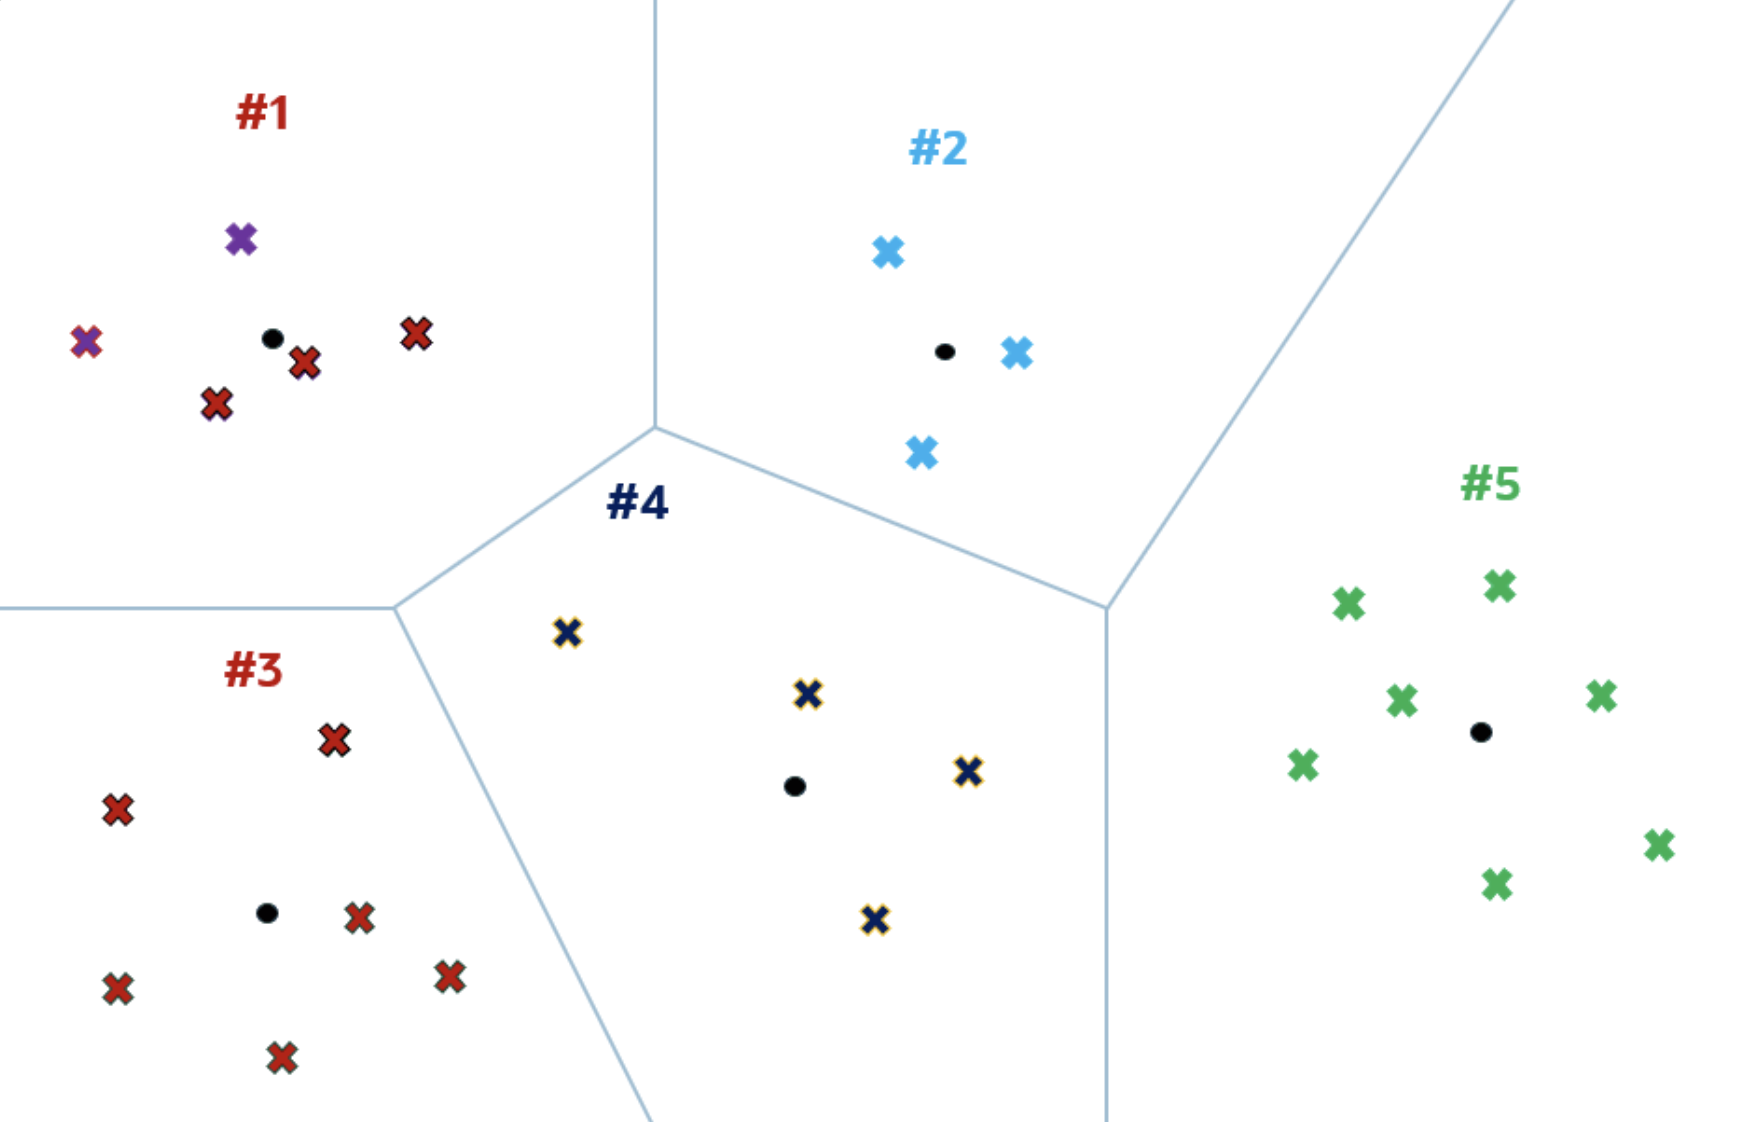
\includegraphics[width=0.72\textwidth]{./assets/voronoi_cells.png}
\caption{Example of a vector space partitioned into Voronoi cells. Each cell is associated with one coarse centroid, and each database vector is assigned to the inverted list of its closest centroid. Adapted from Oracle Database documentation \cite{oracle_ivf_flat}.}
\label{fig:voronoi-cells}
\end{figure}

Search is divided into a coarse quantization stage and a fine-search stage over the selected inverted lists \cite{faiss}. During coarse search, the query is compared with the \(N_{\mathrm{list}}\) centroids. The closest \(N_{\mathrm{probe}}\) centroids are selected. Fine search then evaluates the vectors contained in the corresponding inverted lists:
\begin{equation}
\mathcal{D}_{\mathrm{candidate}}(\mathbf{q})=\bigcup_{j\in P(\mathbf{q})}L_j,
\end{equation}
where \(P(\mathbf{q})\) is the set of lists selected for query \(\mathbf{q}\) and
\begin{equation}
\left|P(\mathbf{q})\right|=N_{\mathrm{probe}}.
\end{equation}
\newline
The main IVF parameters are:
\begin{itemize}
\item \(N_{\mathrm{list}}\), the number of coarse clusters or inverted lists into which the dataset is partitioned;
\item \(N_{\mathrm{probe}}\), the number of inverted lists searched for each query.
\end{itemize}

Increasing \(N_{\mathrm{probe}}\) generally increases recall because a larger portion of the dataset is examined, but it also increases execution time and memory traffic. Increasing \(N_{\mathrm{list}}\) produces smaller clusters and can reduce the number of candidates per probed list, although it makes the coarse-search stage more expensive and may produce load imbalance when cluster sizes are not uniform.

The main source of approximation in IVF is the partition-boundary problem. A vector may be very close to the query while belonging to a Voronoi cell whose centroid was not selected during coarse search. In this case, the vector is excluded from the candidate set before its exact distance from the query is computed.

Figure~\ref{fig:ivf-missed-vector} shows a concrete example of this behavior. The dataset is partitioned into five Voronoi cells, and the query \(\mathbf{q}\) belongs to the red cell. The vectors labeled from \(\#1\) to \(\#5\) are the five exact nearest neighbors of the query. Four of these vectors belong to the selected red cell and are evaluated during fine search. However, vector \(\#2\) lies immediately across the boundary in the neighboring blue cell. Because that cell is not probed, vector \(\#2\) is not included in \(\mathcal{D}_{\mathrm{candidate}}(\mathbf{q})\), even though it belongs to the exact top-\(5\) result.

\begin{figure}[htbp]
\centering
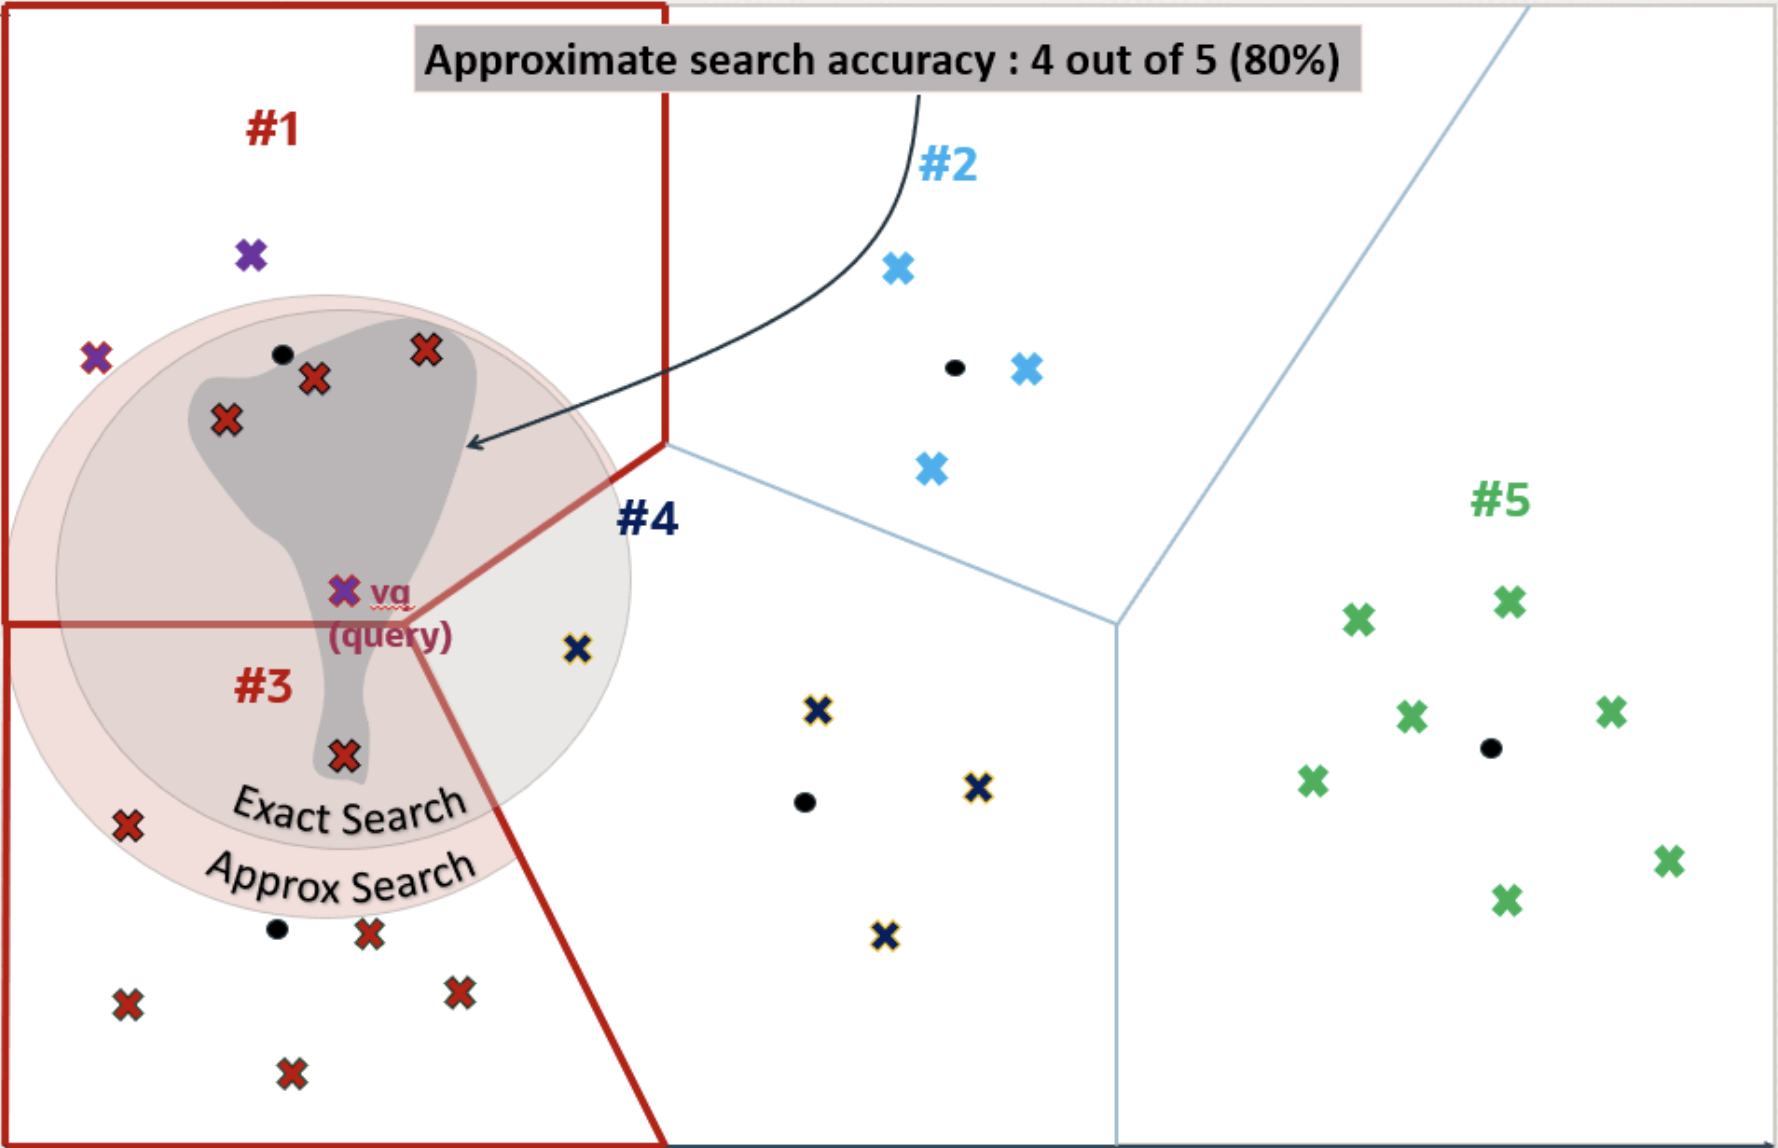
\includegraphics[width=0.95\textwidth]{./assets/ivf_missed_vector.png}
\caption{Example of a missed nearest neighbor in IVF search. The vectors labeled from \(\#1\) to \(\#5\) form the exact top-\(5\) result. Vector \(\#2\) lies in an unprobed neighboring Voronoi cell and is therefore excluded from the approximate result, which retrieves four of the five exact nearest neighbors.}
\label{fig:ivf-missed-vector}
\end{figure}

Using the recall definition introduced in Section~\ref{sec:ann}, the approximate result in Figure~\ref{fig:ivf-missed-vector} achieves
\begin{equation}
\operatorname{Recall@5}=\frac{\left|\operatorname{ANN}_5(\mathbf{q})\cap\operatorname{NN}_5(\mathbf{q})\right|}{5}=\frac{4}{5}=0.8.
\end{equation}

The missed vector is not caused by an inaccurate distance calculation. Its distance is never evaluated because coarse search excludes the inverted list containing it. Increasing \(N_{\mathrm{probe}}\) may include the neighboring blue cell and recover vector \(\#2\), but it also increases the number of candidate vectors, distance computations, and memory transfers.

Despite this limitation, IVF exposes substantial parallelism. Coarse distances can be computed independently, selected clusters can be searched concurrently, and distance computation within each cluster is regular. Vectors in an inverted list can also be stored contiguously, providing more predictable memory accesses than pointer-based index structures.

IVF-Flat stores the original vectors inside each inverted list. Consequently, the distances evaluated during fine search are exact with respect to the selected candidates; approximation is introduced only by the coarse partitioning and the selection of a subset of the lists.

Several extensions reduce the memory footprint or the amount of fine-search work. IVF-PQ stores product-quantized codes instead of complete vectors, while related methods compute approximate distances in the compressed domain \cite{faiss}. ScaNN combines search-space pruning with quantization techniques, including anisotropic vector quantization for maximum inner-product search \cite{scann}. These approaches can significantly reduce memory traffic but introduce additional codebook lookups, approximate-distance computations, and often a re-ranking stage.

\section{Graph-Based Indexes}
\label{sec:graph-indexes}

Graph-based ANN methods represent dataset vectors as vertices of a proximity graph. Edges connect vectors that are close according to the selected metric. At query time, search starts from one or more entry vertices and repeatedly moves toward neighboring vertices that appear closer to the query.

Unlike IVF, graph search does not define a fixed set of spatial partitions to visit. The visited region is determined dynamically by the distances observed during traversal. This can provide high recall while evaluating a relatively small fraction of the dataset, including points located across coarse partition boundaries.

Graph-based methods are particularly effective on CPUs because CPUs provide efficient branch execution, cache hierarchies optimized for irregular access, and SIMD instructions for computing distances between a query and a small set of candidate vectors. Their main disadvantage is that traversal is data-dependent: different queries visit different vertices, perform different numbers of iterations, and access different memory locations.

The two representative graph-based approaches considered in this chapter are HNSW, described in Section~\ref{subsec:hnsw}, and NGT, described in Section~\ref{subsec:ngt}.

\subsection{HNSW: Hierarchical Navigable Small World}
\label{subsec:hnsw}

Hierarchical Navigable Small World, or HNSW, organizes proximity connections into multiple layers \cite{hnsw}. The bottom layer contains all indexed vectors, while progressively higher layers contain increasingly sparse subsets.

The level assigned to each vector is selected probabilistically, with the probability of appearing at higher levels decreasing exponentially. This creates a hierarchy conceptually similar to a skip list: upper layers contain long-range connections that allow the search to move rapidly across the dataset, while lower layers provide increasingly local refinement \cite{skiplist}.

Search begins from an entry point in the highest layer. At each level, the algorithm greedily follows neighbors that improve the distance to the query. Once no closer neighbor is found, the search continues from the current vertex in the next lower layer. At the bottom layer, a wider best-first search is performed using a dynamically maintained candidate queue \cite{hnsw}.
\newline
A simplified representation of the search procedure is:
\begin{enumerate}
\item select an entry vertex in the highest graph layer.
\item greedily traverse the current layer toward the query.
\item use the resulting vertex as the entry point for the layer below.
\item at the bottom layer, maintain a bounded set of promising candidates.
\item terminate when the remaining candidates cannot improve the current result set.
\end{enumerate}

Figure~\ref{fig:hnsw} illustrates this hierarchical organization. The upper layers contain only a sparse subset of the indexed vectors and provide long-range edges that allow the search to move rapidly toward the region containing the query. After reaching a local minimum in one layer, the search descends to the corresponding vertex in the next denser layer. The final and most detailed exploration is performed in layer \(0\), which contains all indexed vectors. This hierarchy allows HNSW to combine coarse navigation in the upper layers with fine-grained neighbor exploration in the bottom layer.

\begin{figure}[htbp]
\centering
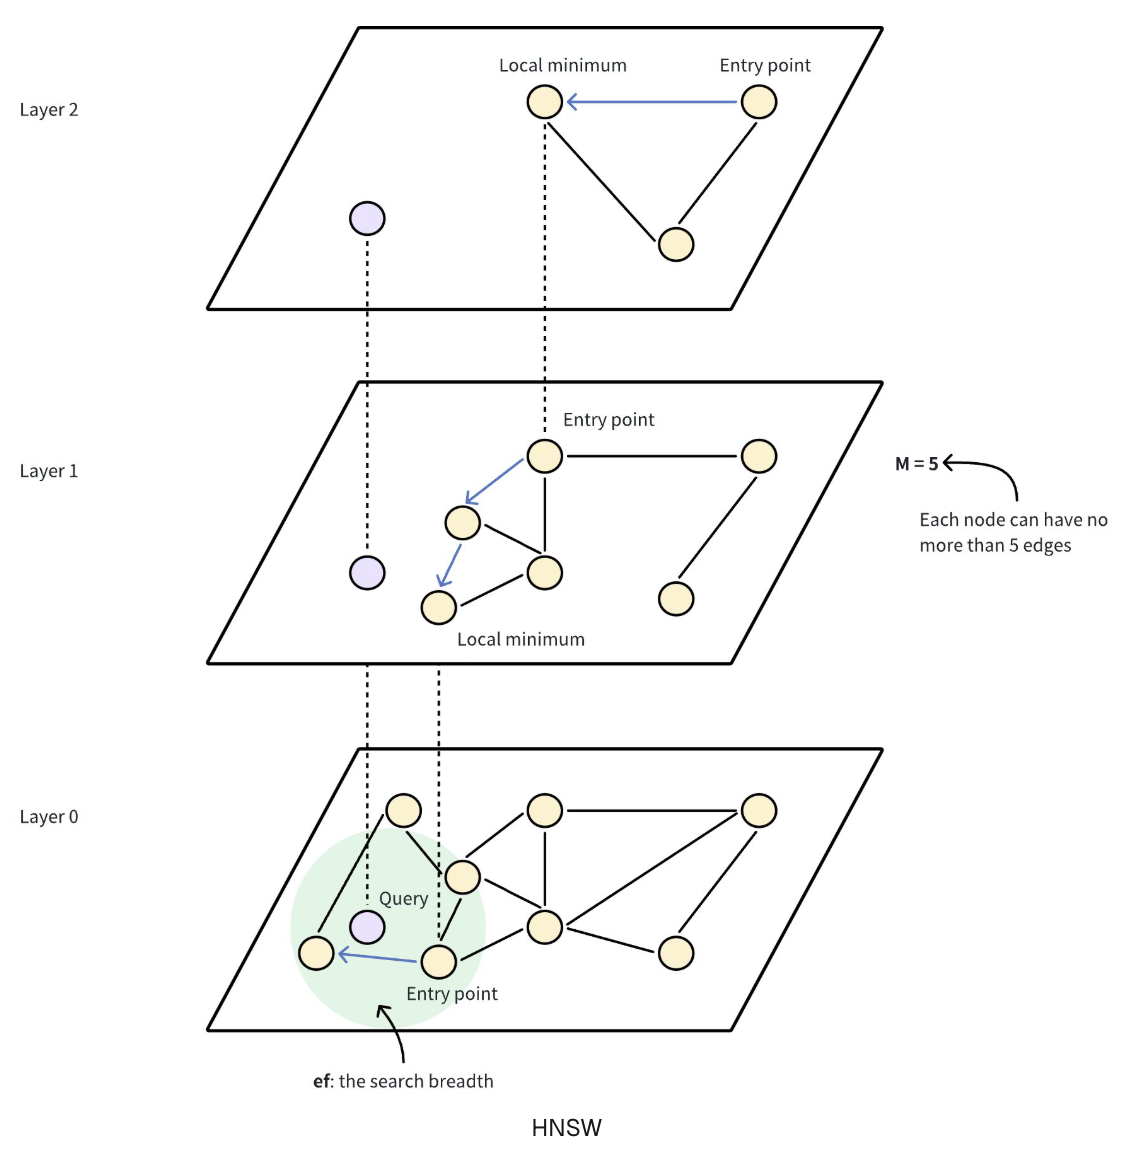
\includegraphics[width=0.78\textwidth]{./assets/hnsw.png}
\caption{Hierarchical organization of an HNSW index. Sparse upper layers provide long-range navigation, while the dense bottom layer supports fine-grained nearest-neighbor search. Adapted from the Milvus HNSW documentation \cite{milvus_hnsw}.}
\label{fig:hnsw}
\end{figure}

The maximum number of connections per vertex and the candidate-list size control the memory, recall, and latency trade-offs. HNSW is known for strong high-recall performance but may require substantial memory because both the original vectors and graph adjacency lists must be stored.
\newline
From an accelerator perspective, HNSW presents several challenges:
\begin{itemize}
\item neighbor addresses depend on the currently visited vertex;
\item adjacency lists and vectors may be distributed across memory;
\item the search frontier and result queue are updated dynamically;
\item different queries follow different paths and terminate after different numbers of steps;
\item visited-set management requires additional random accesses and synchronization.
\end{itemize}

These characteristics do not prevent accelerator implementations, but they make it harder to obtain the regular, high-throughput execution typically associated with dense tensor operations. Unlike the IVF partitioning described in Section~\ref{sec:ivf-background}, HNSW can cross coarse spatial boundaries by traversing graph edges. The consequences of its irregular traversal for Tenstorrent are discussed in Section~\ref{subsec:graph-tt-fit}.

\subsection{NGT: Neighborhood Graph and Tree}
\label{subsec:ngt}

Neighborhood Graph and Tree, or NGT, combines a neighborhood graph with a separate tree-based structure used to obtain good entry points for graph traversal \cite{ngt}. Conceptually, it is similar to HNSW in that both methods first try to move the search toward a promising region of the vector space before performing a more detailed local graph exploration.

The main difference lies in how this initial region is reached. In HNSW, the search uses the hierarchy of the graph itself: it starts from sparse upper layers and progressively descends toward the denser bottom layer. NGT instead uses a separate tree-based structure to locate one or more objects that are expected to be close to the query. These objects are then used as entry vertices for the neighborhood graph.

In this sense, the tree in NGT plays a role similar to the upper layers of HNSW, since both mechanisms reduce the need to begin graph traversal from an arbitrary point. However, the two approaches are structurally different. HNSW integrates coarse navigation and local search into a single hierarchical graph, whereas NGT separates the initial tree-based localization from the subsequent neighborhood-graph traversal.

Once the entry vertices have been identified, NGT explores the neighborhood graph by maintaining a candidate set ordered according to distance from the query. The most promising unexplored candidate is expanded, its neighboring vertices are evaluated, and sufficiently close neighbors are inserted into the candidate set. This process continues until the termination condition is satisfied, after which the best \(k\) objects found during traversal are returned.

Figure~\ref{fig:ngt-overview} summarizes the search process. The tree first performs a coarse localization of the query and selects the initial graph vertices. The neighborhood graph is then explored from these seeds to progressively refine the candidate set and obtain the approximate nearest neighbors.

\begin{figure}[htbp]
\centering
\begin{tikzpicture}[
node distance=1.3cm,
box/.style={draw, rounded corners, minimum width=5.0cm, minimum height=0.9cm, align=center},
arrow/.style={-{Latex[length=3mm]}, thick}
]
\node[box] (query) {Query vector \(\mathbf{q}\)};
\node[box, below=of query] (tree) {Locate a promising region using the tree};
\node[box, below=of tree] (seed) {Select initial graph vertices};
\node[box, below=of seed] (graph) {Traverse the neighborhood graph};
\node[box, below=of graph] (result) {Approximate top-\(k\) results};
\draw[arrow] (query) -- (tree);
\draw[arrow] (tree) -- (seed);
\draw[arrow] (seed) -- (graph);
\draw[arrow] (graph) -- (result);
\end{tikzpicture}
\caption{High-level NGT search process. The tree first identifies a promising region of the vector space and provides initial graph vertices. The neighborhood graph is then explored from these seeds to refine the search and obtain the approximate nearest neighbors. Original illustration based on \cite{ngt}.}
\label{fig:ngt-overview}
\end{figure}

As with HNSW, NGT can achieve high recall while evaluating only a subset of the dataset. Its execution is nevertheless irregular: the next vertices to visit depend on the query and on the distances observed during traversal. The search therefore involves non-contiguous graph accesses, dynamic candidate-set updates, and branch-dependent control flow. The additional tree traversal introduces another query-dependent stage before neighborhood exploration begins.

For this thesis, HNSW and NGT illustrate a common property of graph-based ANN methods: they reduce the number of distance computations by relying on irregular memory accesses and dynamic traversal decisions. These characteristics differ substantially from the regular, tile-oriented execution model targeted by the Tenstorrent architecture, and their suitability is discussed jointly in Section~\ref{subsec:graph-tt-fit}.

\section{GPU-Specialized ANN Indexes}
\label{sec:gpu-indexes}

GPUs provide high arithmetic throughput and memory bandwidth, making them well-suited to regular batched distance computations. However, efficient ANN search on GPUs requires algorithms that expose sufficient parallelism and avoid frequent divergent branches or fine-grained dynamic memory operations.

\subsection{GPU IVF and Faiss}
\label{subsec:gpu-faiss}

IVF naturally maps to GPU execution because many queries, clusters, and candidate vectors can be processed concurrently. GPU implementations can parallelize both the coarse centroid comparisons and the fine-search distance calculations over selected clusters.

One important difficulty is selecting the smallest or largest \(k\) elements from a large set of candidate distances. A conventional heap performs data-dependent insertions and provides insufficient parallelism for efficient GPU execution.

The GPU implementation presented by Johnson et al.\ in Faiss introduces a register-resident selection method designed around GPU warps \cite{faiss}. Candidate values are processed cooperatively by the threads of a warp, reducing global-memory traffic and avoiding the use of a conventional branch-heavy heap. The method is integrated with brute-force, IVF, and product-quantized search.
\newline
The resulting search pipeline uses the GPU effectively because:
\begin{itemize}
\item distance calculations are independent and data parallel;
\item the same kernel can process large batches of queries;
\item candidate vectors can be read through coalesced or block-oriented memory accesses;
\item selection is performed using warp-level cooperation;
\item intermediate results can remain in registers or shared memory.
\end{itemize}

The Faiss work demonstrates that the top-\(k\) stage, rather than only distance computation, must be designed specifically for the target architecture \cite{faiss}.

\subsection{GPU Graph Search and CAGRA}
\label{subsec:cagra}

Traditional proximity-graph indexes are difficult to execute efficiently on GPUs because each query follows a data-dependent path and maintains its own candidate and visited sets. CAGRA addresses this problem through a graph structure and traversal strategy designed specifically for highly parallel GPU execution \cite{cagra}.

CAGRA demonstrates that graph-based ANN search can be adapted to GPUs, but this requires substantially more than transferring a conventional CPU graph traversal to CUDA. Its design modifies both graph construction and query execution to expose bounded and predictable parallel work.

First, CAGRA constructs a single-layer proximity graph with a fixed out-degree, bounding the amount of work associated with each vertex expansion \cite{cagra}. A bounded degree ensures that expanding one graph vertex always produces a known maximum number of neighbors, allowing their vector distances to be evaluated cooperatively by GPU threads. This is considerably more regular than a graph in which adjacency-list lengths vary arbitrarily.

Second, graph traversal is organized around fixed-capacity candidate and result structures rather than dynamically allocated CPU priority queues. Threads within a GPU block cooperate in expanding candidates, computing distances, filtering previously visited vertices, and updating the candidate set. These structures must fit within the memory and synchronization model available to a GPU thread block.

Third, visited-node tracking is implemented using a bounded GPU-oriented structure. Unlike an exact dynamically growing CPU set, this representation accepts limited capacity and possible repeated visits in exchange for predictable memory usage and parallel lookup behavior. The search procedure is therefore designed to tolerate approximation not only in graph traversal but also in auxiliary bookkeeping.

Finally, the stopping policy and the number of expanded candidates are adapted to parallel execution. The algorithm must keep enough work available for the GPU while limiting divergent control flow between queries. These changes show that accelerator graph search requires the graph degree, candidate queue, visited set, work assignment, and termination condition to be co-designed with the target architecture \cite{cagra}.

\subsubsection*{CAGRA versus IVF on GPUs}

Neither CAGRA nor IVF is universally superior on GPUs. The preferable index depends on the required recall, dataset size and distribution, query-batch size, available memory, and index-construction constraints.

IVF exposes regular and highly parallel execution because vectors within each selected inverted list can be read and evaluated in contiguous blocks. Its index structure is comparatively simple, and quantized variants such as IVF-PQ can reduce storage and device-memory bandwidth. However, high-recall search may require probing many inverted lists. As \(N_{\mathrm{probe}}\) increases, the system evaluates more candidate vectors and approaches the cost of exhaustive search.

CAGRA instead uses graph connectivity to navigate toward promising areas of the dataset without scanning entire clusters. Its fixed-degree graph and cooperative GPU traversal are designed to provide high throughput at high recall \cite{cagra}. This advantage comes with additional graph storage, more complex index construction, indirect vector accesses, and candidate and visited-state structures that must be managed during traversal.

CAGRA is therefore particularly attractive for high-recall, memory-resident GPU workloads when graph construction and storage costs are acceptable. IVF remains attractive when regular execution, simpler construction, predictable partitioning, support for datasets larger than available accelerator memory, or compatibility with compression are more important. The comparison is implementation-dependent: optimized quantized IVF variants may outperform graph-based methods at some high-recall operating points \cite{ivf_rabitq_gpu}.

The approach used by CAGRA is highly relevant when considering graph search on Tenstorrent. It shows that accelerator execution is possible, but a direct port of a CPU graph algorithm is unlikely to be efficient. The graph structure, memory layout, candidate management, and traversal strategy must all be redesigned around the target accelerator.

\section{Tenstorrent Architecture and Programming Model}
\label{sec:tt-architecture}

Tenstorrent processors are spatial many-core accelerators whose Tensix cores
form a two-dimensional grid connected through one or more Networks-on-Chip.
Rather than relying primarily on hardware-managed caches and general-purpose
threads, the programming model gives the developer explicit control over data
placement, movement, core assignment, and synchronization.

Figure~\ref{fig:tensix-core} shows the main components of a Tensix core. A core combines local L1 SRAM, RISC-V processors responsible for data movement and kernel control, and specialized compute engines. The data-movement processors issue transfers through the NoC, while the compute path includes a matrix engine for tile-oriented operations and a vector engine for element-wise and special-function operations. The local SRAM stores circular buffers, input and output tiles, intermediate values, runtime metadata, and other kernel state. Consequently, performance depends not only on arithmetic throughput but also on how effectively computation and data movement are pipelined through the limited local-memory capacity.

\begin{figure}[htbp]
\centering
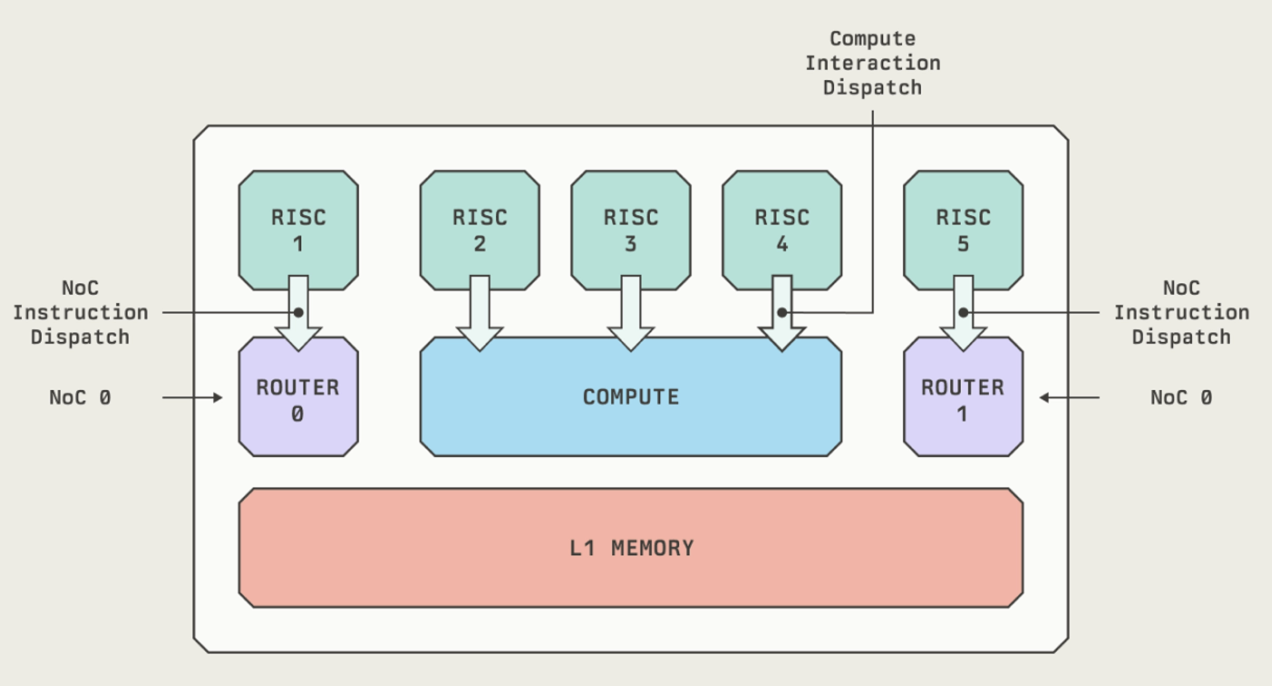
\includegraphics[width=0.82\textwidth]{./assets/tensix.png}
\caption{Simplified organization of a Tensix core, including its RISC-V control and data-movement processors, local L1 SRAM, NoC interfaces, and specialized compute engines. Adapted from the Tenstorrent architecture and TT-Metalium documentation \cite{tenstorrent_metalium_architecture}.}
\label{fig:tensix-core}
\end{figure}

Tenstorrent provides several programming layers with different levels of abstraction. At the highest level considered here, TT-NN provides a Python interface and a library of common tensor and machine-learning operations. It is suitable when an application can be expressed using operations already provided by the library, allowing the runtime to manage much of the device configuration and tensor placement.

TT-Lang provides an intermediate programming layer between TT-NN and TT-Metalium. It is a Python-based domain-specific language for implementing custom Tenstorrent operations while retaining explicit control over data movement, synchronization, and inter-core communication. It provides higher-level constructs such as tensor slices, blocks, and pipes, while remaining more flexible than the predefined operations available in TT-NN. TT-Lang was under active development during this work, and the implementation presented in this thesis was developed directly using TT-Metalium.

TT-Metalium is the lower-level C++ programming interface used to define programs, allocate buffers, select Tensix cores, configure circular buffers, compile kernels, set runtime arguments, and explicitly schedule data movement. TT-Metalium exposes the architecture in sufficient detail to implement non-standard operations such as the ANN kernels developed in this thesis. A typical operation is built from reader, compute, and writer kernels and is first developed for one Tensix core before being distributed across multiple cores or devices.

TT-LLK, or the Low-Level Kernel layer, contains architecture-specific implementations and interfaces for the underlying Tensix compute engines. TT-Metalium compute APIs are commonly built on these lower-level kernels, while direct modification or extension of TT-LLK may be required when the available operations do not expose a needed hardware primitive. In this thesis, the limitations of the available top-\(k\), comparison, and data-manipulation primitives influence which ANN algorithms can be implemented efficiently.

The software stack can therefore be viewed as
\begin{equation}
\text{TT-NN}\rightarrow\text{TT-Lang}\rightarrow\text{TT-Metalium}\rightarrow\text{TT-LLK}\rightarrow\text{Tensix hardware},
\end{equation}
where moving downward provides greater architectural control but also requires more explicit management of memory, synchronization, tilization, and kernel execution.

Most computation on a Tensix core is performed on tiles. The standard tile is a \(32\times32\) block whose elements share the same data type. Tensors whose final dimensions are not multiples of the tile dimensions generally require padding or a different supported layout.
\newline
The relevant memory hierarchy includes:
\begin{itemize}
\item off-chip device DRAM, which provides the capacity required for large tensors and indexes;
\item local L1 SRAM associated with each Tensix core, which provides lower-latency storage for tiles, intermediate values, and circular buffers;
\item explicit transfers over the Network-on-Chip between DRAM interfaces and Tensix cores or among Tensix cores.
\end{itemize}

Data in DRAM is not accessed through a transparent cache. Device kernels explicitly request transfers using the NoC data-movement APIs. Therefore, efficient execution depends strongly on the regularity of the memory-access pattern, the size of each transfer, and the placement of data relative to the cores that consume it.
\newline
A typical TT-Metalium program uses three kinds of kernels:
\begin{itemize}
\item a reader kernel, responsible for transferring input data into local buffers;
\item a compute kernel, which operates on tiles using the Tensix compute engine;
\item a writer kernel, responsible for transferring results to their final location.
\end{itemize}

These kernels communicate through circular buffers in local SRAM. Circular buffers implement a producer--consumer pipeline: a reader reserves space and pushes input tiles, the compute kernel waits for available tiles and produces outputs, and the writer waits for output tiles before transferring them. Double buffering can overlap data movement with computation.
\newline
This execution model is particularly effective for workloads with:
\begin{itemize}
\item regular tile-based computation;
\item statically partitionable work;
\item predictable data movement;
\item contiguous or block-oriented memory accesses;
\item sufficient work per transferred tile;
\item opportunities for batching and data reuse.
\end{itemize}

Conversely, workloads dominated by pointer chasing, fine-grained random access, dynamically sized data structures, and query-dependent control flow are more difficult to map efficiently. Such workloads may still be implementable, but often require transformations that increase the amount of work, memory traffic, or synchronization.

\section{Related Work}
\label{sec:related-work}

\subsection{ANN Search on Specialized Accelerators}

Beyond CPUs and GPUs, ANN search has been mapped to FPGAs, TPUs, and dedicated hardware. FANNS co-designs the parameters of an IVF-PQ index and an FPGA accelerator for a given dataset and recall target, reporting speed-ups of up to 23.0 times over FPGA baselines and 37.2 times over CPU baselines \cite{fanns}. TPU-KNN instead performs nearest-neighbor search on TPUs at close to peak FLOP/s: guided by a performance model that accounts for both memory and instruction bottlenecks, it replaces index traversal with dense matrix computation and outperforms GPU methods at similar recall \cite{tpu_knn}. ANNA proposes a specialized architecture for product-quantization-based ANN search \cite{anna}. TPU-KNN is the closest in spirit to this thesis: both target a matrix-oriented accelerator and trade additional arithmetic for regular, tile-friendly execution.

\subsection{Applications of Tenstorrent Hardware}

Published studies of Tenstorrent hardware beyond machine-learning inference have focused on dense numerical kernels. On the Grayskull e150, a Jacobi stencil reached performance similar to a Xeon Platinum CPU while using about five times less energy \cite{brown_grayskull_stencil}. On the Wormhole, a two-dimensional FFT ran slower than a 24-core Xeon Platinum CPU but consumed about 2.8 times less energy \cite{brown_wormhole_fft}, and a gravitational \(N\)-body simulation on a Wormhole n300 achieved more than a twofold speed-up and about twofold energy savings over an optimized CPU implementation \cite{almerol_wormhole_nbody}.

These workloads have regular, data-independent access patterns. ANN search differs in that the data accessed by each query depends on a data-dependent list selection, list sizes are irregular, and results require a top-\(k\) selection rather than a dense output. To the best of our knowledge, no approximate nearest-neighbor search implementation for Tenstorrent hardware has been published, and this thesis presents the first.

\section{Suitability of ANN Indexes for Tenstorrent}
\label{sec:index-suitability}

The suitability of an ANN index for Tenstorrent depends on more than its algorithmic complexity. An index that performs fewer distance computations may still execute inefficiently if it requires irregular memory accesses, dynamic priority queues, or frequent synchronization.
\newline
The principal criteria considered in this thesis are:
\begin{enumerate}
\item regularity of the computation;
\item spatial locality of the indexed vectors;
\item predictability and granularity of DRAM transfers;
\item ability to batch multiple queries;
\item amount of query-dependent control flow;
\item size and dynamism of intermediate data structures;
\item possibility of statically distributing work across Tensix cores.
\end{enumerate}

\subsection{IVF-Flat}
\label{subsec:ivf-tt-fit}

IVF-Flat provides the most natural mapping among the considered ANN indexes. Both coarse and fine search are dominated by independent vector-distance calculations. The centroids form a dense matrix, while vectors assigned to the same cluster can be stored in contiguous regions of device DRAM.

Coarse search can be performed for a batch of queries by comparing a \(32\)-query tile with tiles containing the centroid vectors. This arrangement matches the native tile dimensions and allows the queries to be reused while centroid blocks are streamed through the compute cores.

Fine search can then be partitioned by assigning selected clusters or groups of clusters to different workers. Each worker reads contiguous vector blocks, computes their distances from the corresponding queries, and produces a local set of candidates. Partial results are subsequently merged.

The implementation developed in this thesis does not treat each query--cluster pair as a completely independent GPU-style task. Instead, work is organized around batches of up to \(32\) queries and the union of the clusters selected for those queries. This allows the data layout and computation to remain compatible with tile-based execution.
\newline
The main difficulties are:
\begin{itemize}
\item inverted lists have different numbers of vectors;
\item different queries may select overlapping or disjoint sets of lists;
\item the amount of work increases with \(N_{\mathrm{probe}}\);
\item workers may receive unequal candidate-set sizes;
\item local candidate sets must be merged into a global top-\(k\);
\item cluster metadata and worker schedules must be generated and transferred efficiently.
\end{itemize}

These issues require explicit scheduling and load balancing, but the dominant computation remains regular enough to benefit from the Tensix architecture. As discussed in Section~\ref{sec:ivf-flat-selection}, this combination of properties made IVF-Flat the index selected for the implementation developed in this thesis.

This section provides only the architectural motivation for mapping IVF-Flat to Tenstorrent. The complete implementation, including the data layout, query batching, coarse-search kernels, fine-search scheduling, top-\(k\) processing, and host--device interaction, is described in Chapter~\ref{chap:design-implementation}.

\subsection{Graph-Based Indexes}
\label{subsec:graph-tt-fit}

Graph-based indexes are less naturally aligned with the current Tenstorrent programming model. To expand one graph vertex, the implementation must first retrieve its adjacency list and then fetch the vectors associated with the listed neighbors. The addresses of these vectors are known only after the current vertex has been processed.

The resulting memory-access sequence is therefore indirect:
\begin{equation}
\text{vertex}\rightarrow\text{adjacency list}\rightarrow\text{neighbor identifiers}\rightarrow\text{neighbor vectors}.
\end{equation}

The neighbor vectors are not guaranteed to be contiguous in DRAM. Transferring complete tiles may consequently fetch vectors that are not needed by the current traversal. Alternatively, issuing small row-major transfers can reduce the transferred volume but may underutilize DRAM and NoC bandwidth.
\newline
Graph traversal also requires:
\begin{itemize}
\item a dynamic candidate queue ordered by distance;
\item a bounded result set;
\item a representation of the previously visited vertices;
\item repeated termination checks;
\item synchronization when multiple workers cooperate on one query.
\end{itemize}

Batching does not completely solve the problem because different queries may visit unrelated regions and execute different numbers of iterations. Some queries may therefore finish while others continue traversing the graph, reducing the utilization of cores assigned to the batch.

Graph indexes should therefore not be described as impossible to implement on Tenstorrent. A possible implementation could use fixed-degree graphs, fixed-capacity candidate buffers, batched frontier expansion, and approximate visited sets. However, this would require a substantial redesign similar in spirit to CAGRA and was beyond the scope of this thesis.

\subsection{CAGRA}
\label{subsec:cagra-tt-fit}

CAGRA is designed for GPU execution, but its GPU-oriented design does not automatically make it efficient on Tenstorrent. Both architectures exploit parallelism, but their execution models and memory hierarchies differ.

The fixed graph degree in CAGRA is beneficial because it bounds the amount of work associated with one vertex expansion. Groups of \(32\) neighbors could, in principle, be arranged to match a Tensix tile dimension. Nevertheless, the identifiers still refer to vectors that may be located in unrelated DRAM regions. Efficiently gathering those vectors remains difficult.

The candidate queue and visited-state structure also require careful consideration. A GPU implementation can use registers, shared memory, and thread-block cooperation to maintain bounded structures. On Tenstorrent, each Tensix core has a limited amount of L1 SRAM that is also used for circular buffers, input tiles, output tiles, metadata, and program state. Reserving a large per-query candidate or visited structure would reduce the space available for double buffering and data reuse.

Placing these structures in device DRAM would increase capacity but introduce additional NoC transfers and latency on every graph iteration. Distributing them over multiple Tensix cores would require synchronization and ownership rules for concurrent updates.
\newline
A Tenstorrent-oriented graph index could still be explored in future work, for example by combining:
\begin{itemize}
\item a fixed graph degree compatible with tile dimensions;
\item batched expansion of several query frontiers;
\item a compact probabilistic visited-state representation;
\item graph reordering to improve spatial locality;
\item bounded iteration counts and fixed-capacity candidate queues.
\end{itemize}

Another possible Tenstorrent-specific design would group multiple dataset vectors into one logical graph vertex. For example, each logical vertex could contain a block of \(32\) vectors, allowing one block to align with a native tile dimension and enabling the distance calculations for those vectors to be performed together. The graph connecting these blocks could use a small fixed degree, such as four outgoing edges. Most edges could connect blocks representing nearby regions, while one edge could provide a longer-range connection intended to improve global navigability.

This organization would reduce the granularity mismatch between conventional graph traversal and tile-oriented execution. Fetching one graph vertex would provide enough vectors to occupy the compute engine, and a fixed low degree would bound the number of successor blocks considered during each expansion. It could also reduce adjacency metadata compared with representing every vector as an independent graph node.

However, grouping vectors changes the semantics of the graph. The \(32\) vectors contained in one block may not all be equally close to one another or to the query, and selecting a block may require evaluating many vectors that would not have been visited by a conventional graph search. Constructing balanced blocks with both good internal locality and useful inter-block edges would therefore become a separate indexing problem. The search would still require a candidate queue, a visited-block representation, query-dependent termination, and indirect DRAM accesses to successor blocks. Long-range edges would also need to be constructed carefully to improve navigability without causing excessive exploration. This design may better match Tensix execution than a conventional per-vector graph, but it does not eliminate the fundamental control-flow and memory-access challenges of graph-based ANN search.

Such an implementation would therefore constitute a separate research project rather than a direct extension of the IVF pipeline.

\subsection{IVF-PQ and Quantized Indexes}
\label{subsec:quantized-tt-fit}

Product quantization \cite{jegou_pq} divides a vector into \(m\) sub-vectors and replaces each sub-vector with the identifier of its closest codeword. A database vector is therefore represented using a short sequence of codebook indices rather than its original coordinates. Figure~\ref{fig:ivf-pq} illustrates this process: the original vector is divided into independent subspaces, each sub-vector is mapped to a codeword from its corresponding codebook, and the resulting codeword identifiers form the compressed representation.

\begin{figure}[htbp]
\centering
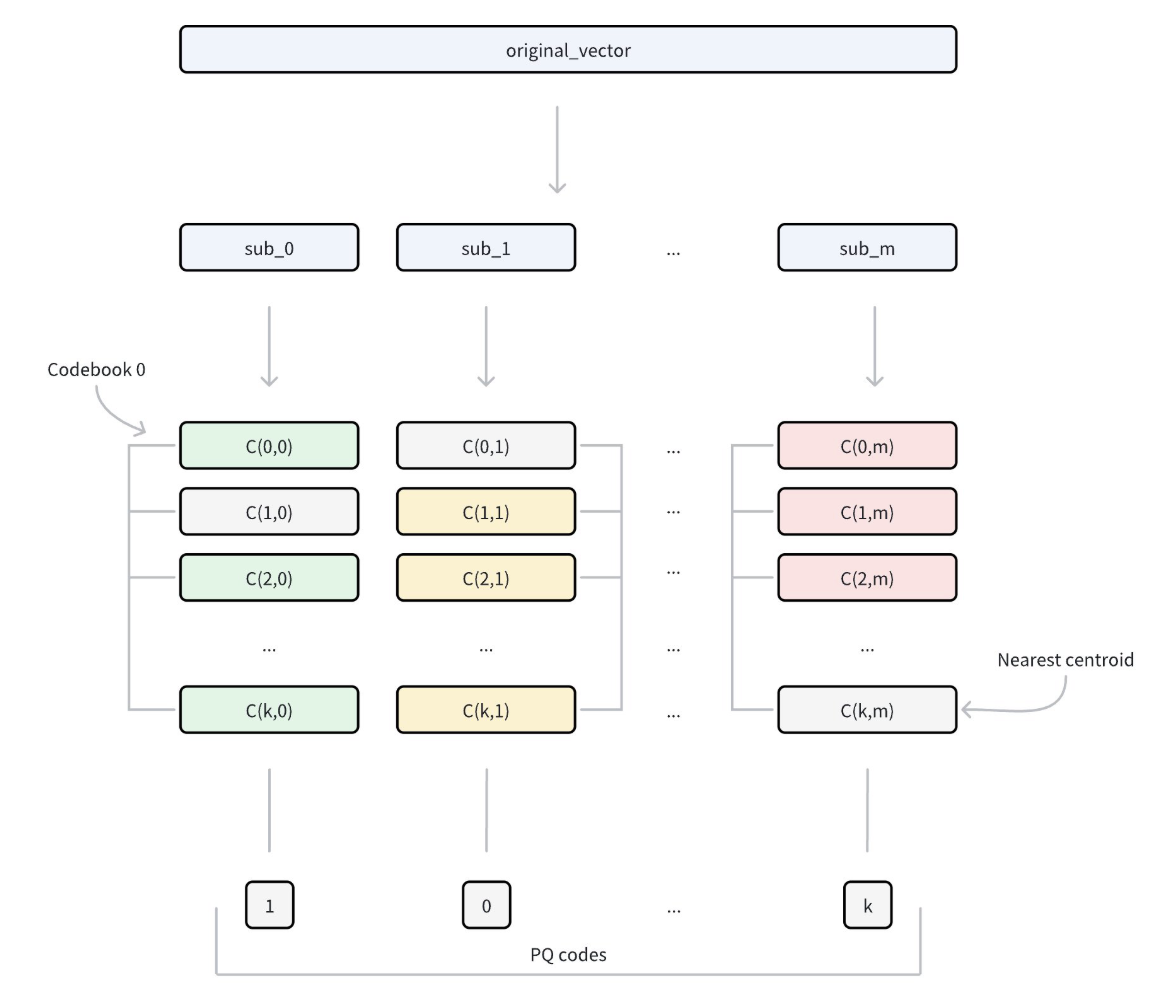
\includegraphics[width=0.82\textwidth]{./assets/ivfpq.png}
\caption{Overview of product quantization within an IVF-PQ index. Each vector is divided into sub-vectors and represented by codeword identifiers from independently trained subspace codebooks. Approximate distances are computed by accumulating values from query-specific lookup tables. Adapted from the Milvus IVF-PQ documentation \cite{milvus_ivfpq}.}
\label{fig:ivf-pq}
\end{figure}

For a query, lookup tables containing the distance between each query sub-vector and each codeword can be precomputed. As shown in Figure~\ref{fig:ivf-pq}, the approximate distance to a compressed database vector is obtained by using its codeword identifiers to select one value from each lookup table and summing the selected values.
\newline
IVF-PQ preserves the coarse partitioning of IVF and therefore retains many of its favorable properties:
\begin{itemize}
\item encoded vectors can be stored contiguously within each inverted list;
\item many codes can be evaluated independently;
\item the reduced representation lowers DRAM capacity and bandwidth requirements;
\item coarse search and cluster scheduling can reuse the IVF-Flat design.
\end{itemize}

The difficulty is not that the original vector must be fetched for every candidate. During the approximate stage, distances can be computed directly from the compressed codes. Original vectors are required only when an optional exact re-ranking stage is performed.
\newline
The main implementation challenges on Tenstorrent are:
\begin{itemize}
\item implementing efficient small-table lookups;
\item decoding packed codeword identifiers;
\item supporting integer and mixed-precision accumulation;
\item arranging codebooks for efficient local reuse;
\item gathering original vectors if exact re-ranking is enabled.
\end{itemize}

Although IVF-PQ reduces the amount of data stored in DRAM, its fine-search access pattern is less suitable for the current Tenstorrent implementation than the sequential reading of full vectors used by IVF-Flat. Each candidate code contains several packed codeword identifiers, and evaluating it requires decoding those identifiers and performing multiple indexed accesses into relatively small distance tables. These gathers are regular at the algorithmic level but do not directly correspond to the dense tile operations for which the available Tensix compute primitives are optimized.

The lookup tables could be copied into local SRAM and reused across many candidates, but each Tensix core would then need sufficient local capacity for the tables, circular buffers, candidate codes, intermediate distances, and top-\(k\) state. If the tables or decoded data cannot remain local, repeated accesses through device memory or the NoC may offset part of the bandwidth reduction obtained from compression. Packed-code extraction and mixed-precision accumulation would also require additional low-level kernels.

For these reasons, IVF-PQ was not considered a promising first index for the current implementation. This conclusion concerns its mapping to the present Tenstorrent software stack rather than the general efficiency of IVF-PQ. A specialized implementation with local lookup-table reuse, efficient packed-code decoding, and dedicated quantized-distance kernels could make IVF-PQ attractive in future work.

\subsection{ScaNN}
\label{subsec:scann-tt-fit}

ScaNN combines partitioning, quantization, and re-ranking. Its anisotropic quantization objective gives greater importance to preserving components of the quantization residual that have a larger effect on the inner product \cite{scann}.
\newline
A typical ScaNN-style search pipeline combines partition-based pruning, compressed candidate scoring, candidate selection, and optional exact re-ranking \cite{scann}:
\begin{enumerate}
\item partition-based pruning of the search space;
\item approximate scoring of a comparatively large candidate set using highly compressed representations;
\item selection of a sufficiently large set of promising candidates;
\item re-ranking of those candidates using their original vectors to obtain the final top-\(k\) results.
\end{enumerate}

The partitioning and approximate-scoring stages offer parallelism and could potentially be mapped to Tensix cores. However, an efficient implementation would require optimized quantized-distance kernels and a sufficiently large intermediate candidate selection.

In the implementation considered in this thesis, the available top-\(k\) primitive from TT-LLK and the local-memory budget constrain the number of candidates that can be maintained efficiently inside one device program. Re-ranking also requires gathering original vectors whose identifiers were produced by the compressed search stage. Unless the dataset is reordered or the selected identifiers exhibit locality, these vectors may be distributed across device DRAM.

These issues do not make ScaNN fundamentally incompatible with Tenstorrent. They indicate that an efficient implementation would require additional support for large candidate selection, quantized lookups, and batched vector gathering. For this reason, ScaNN was considered beyond the scope of the first Tenstorrent ANN implementation.

\section{Motivation for Selecting IVF-Flat}
\label{sec:ivf-flat-selection}

Section~\ref{sec:index-suitability} compared IVF-Flat, graph-based indexes, CAGRA, IVF-PQ, and ScaNN against the same set of criteria: regularity of computation, spatial locality, DRAM-transfer granularity, batchability, query-dependent control flow, and the possibility of static work distribution. IVF-Flat was the only index for which all of these criteria were favorable without requiring a substantial architectural redesign, which is why it was selected for the implementation developed in this thesis.

Two further points reinforced this choice. First, IVF-Flat avoids compression-related approximation during candidate scoring: once a list has been selected, its vectors are compared with the query using their original representation. This simplifies correctness validation and allows the effects of \(N_{\mathrm{list}}\), \(N_{\mathrm{probe}}\), scheduling, and data movement to be studied directly without conflating them with quantization error.

Second, IVF still exposes challenges representative of real accelerator systems, including variable cluster sizes, load balancing, host-side scheduling, DRAM placement, NoC traffic, local top-\(k\) selection, and result merging, without requiring the fully dynamic execution model of graph-based search.

Table~\ref{tab:ann-index-summary} summarizes the principal trade-offs of the index families considered in this chapter.

\begin{table}[htbp]
\centering
\caption{Summary of the ANN indexes considered and their qualitative suitability for the current Tenstorrent programming model.}
\label{tab:ann-index-summary}
\small
\setlength{\tabcolsep}{4pt}
\renewcommand{\arraystretch}{1.15}
\begin{tabular}{p{1.6cm}p{2.5cm}p{2.7cm}p{3.7cm}}
\toprule
Index & Main advantage & Main limitation & Tenstorrent suitability \\
\midrule
Flat & Regular exhaustive computation & Linear work in dataset size & Regular, but excessively expensive at scale \\
IVF-Flat & Contiguous candidate scans and tunable recall & May miss vectors in unprobed cells & High; selected for this thesis \\
HNSW & High recall with relatively few distance evaluations & Irregular traversal and substantial graph state & Low without substantial redesign \\
NGT & Tree-based seeding followed by graph refinement & Dynamic traversal and indirect memory accesses & Low without substantial redesign \\
CAGRA & GPU-oriented high-recall graph search & Complex traversal state and indirect accesses & Potentially feasible with a TT-specific redesign \\
IVF-PQ & Reduced storage and memory traffic & Packed decoding and lookup-table accesses & Moderate, but difficult with current primitives \\
ScaNN & Effective pruning, quantization, and re-ranking & Large intermediate selection and irregular re-ranking & Moderate to low with the current software stack \\
\bottomrule
\end{tabular}
\end{table}

The selection of IVF-Flat should not be interpreted as evidence that other ANN indexes cannot execute on Tenstorrent. Instead, IVF-Flat is the index whose computation, memory layout, and scheduling requirements most directly match the capabilities of the current architecture and software stack. It provides a suitable starting point for studying the feasibility, performance, energy efficiency, and bottlenecks of ANN search on Tenstorrent hardware. Its complete implementation is presented in Chapter~\ref{chap:design-implementation}.

\cleardoublepage
